\subsection{Product perspective}
Our product is an ecosystem of applications that are designed from scratch to accomplish different purposes.
The main goal of the system in general is to collect registered users' data, make them available to third parties and offer monitoring services to the end user.

The system is designed to be a set of three subsystems interacting with each other, as shown in the following diagram:

\begin{figure}[h!]
	\centering
	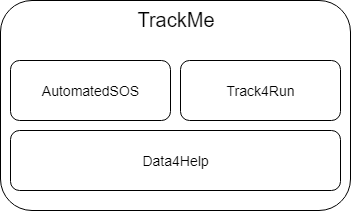
\includegraphics[scale = 0.70]{Images/general_structure.png}\\[1.0 cm]
\end{figure}

In particular, Data4Help is the underlying backbone of our system that collects data from end users and makes it available to third party applications. 

The other two subsystems are built on top of Data4Help and provide to the user different services: AutomatedSOS offers an automated way of calling an ambulance in case of emergency, while Track4Run gives to the end users a platform to organize and participate to run events.

The following subsections give a more detailed analysis of the domain of each subsystem and are accompaigned with the corresponding class diagrams. The aim of these diagrams is to identify the main actors and components of the subsystems and the relationship between them.
 
 \newpage
 
\subsubsection{Data4Help}
Data4Help is meant to be a stand-alone system which works as a gateway between user data producers and third parties, which are data consumers. The central actor of this system is the user.

Each user can configure multiple data sources, each of which can collect different parameters that collectively form the user's data. On the other hand, third parties can make some data requests, that can be targeted to a single user's data or a group of data.

These requests can be of two types: subscriptions, which will cause the third party to be updated whenever the chosen data set changes, or single requests.

Bearing these considerations in mind, the following diagram is given to better describe the domain of the application:

\begin{figure}[h!]
	\centering
	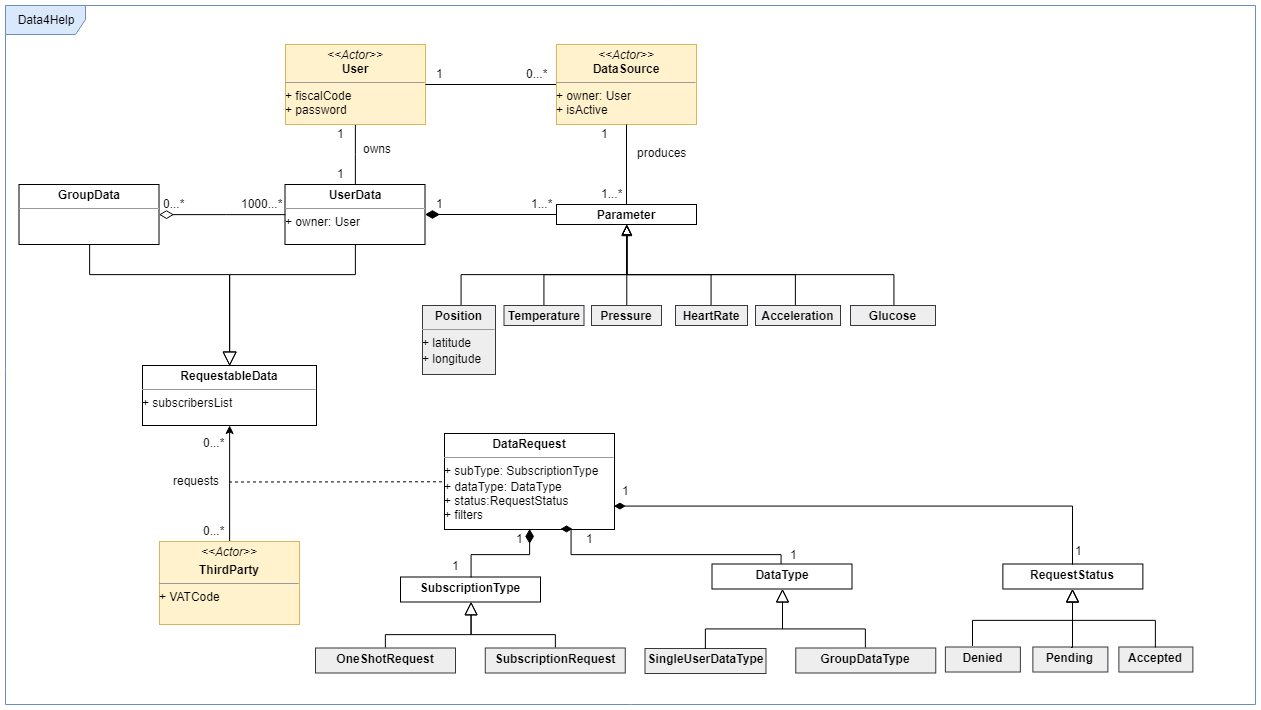
\includegraphics[width = \linewidth] {../Diagrams/ClassDiagram-General.png}\\[1.0 cm]
\end{figure}

Please note that the parameter types listed here are the most commonly used in many kind of applications, but this doesn't exclude that more parameter types can be added in future phases.
\newpage

\subsubsection{AutomatedSOS}
Differently from the previous one, AutomatedSOS is an application which relies on other systems, such as an Ambulance API and Data4Help, to provide a specific service to the end customer. 
The offered service is a monitoring system for Data4Help users, in which some threshold values can be set for each vital parameters. The passing of the threshold by one of these parameters will cause the system to call an ambulance.

In this perspective, the AutomatedSOS system can be seen as one of the third parties of the previous diagram: for each new user, it makes a subscription request for the data of that user to the Data4Help system

\begin{figure}[h!]
	\centering
	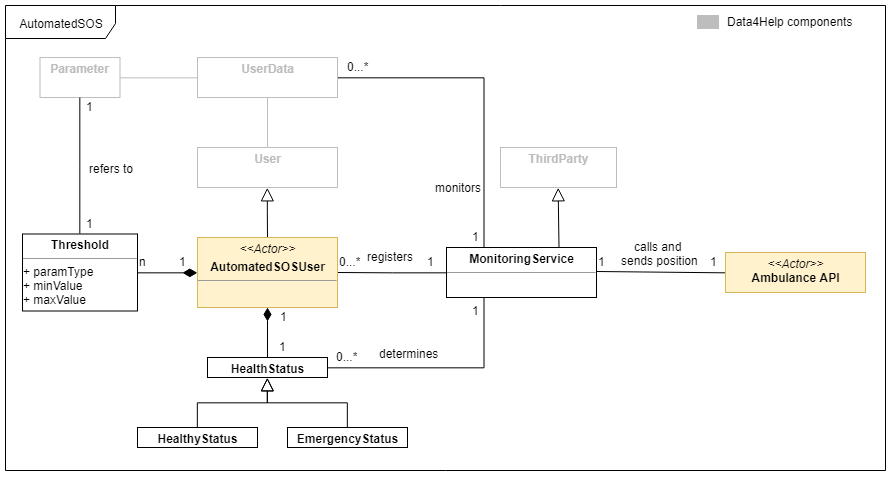
\includegraphics[width = \linewidth] {../Diagrams/ClassDiagram-AutomatedSOS.png}\\[1.0 cm]
\end{figure}

\newpage
\subsubsection{Track4Run}
Like AutomatedSOS, Track4Run is an application that uses Data4Help to monitor some of its users, in particular the runners who participate to run event.
These run events are created and managed by organizers. On the other hand, spectators can see the position of the runners by using the dedicated service.

\begin{figure}[h!]
	\centering
	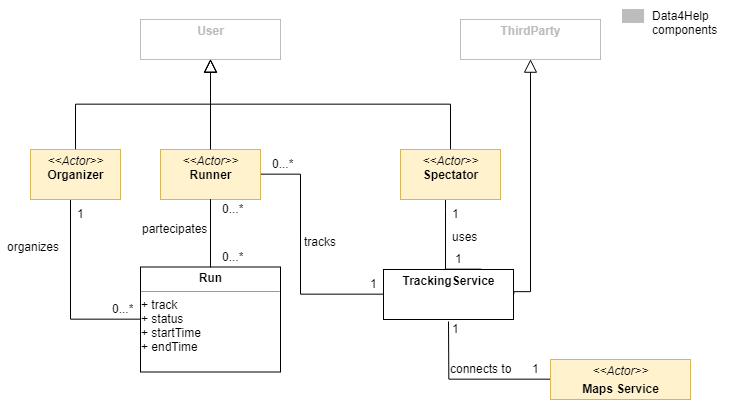
\includegraphics[width = \linewidth] {../Diagrams/ClassDiagram-Track4Run.png}\\[1.0 cm]
\end{figure}
	
\subsection{Product functions}
Considering all the goals that the proposed system has to accomplish, an additional and more detailed description is here provided for the main functions that each subsystem has to accomplish.

\subsubsection{Data4Help - User Data Acquisition}
Data acquisition is the focus of Data4Help and it is also fundamental for all the subsystems built on top of it.

In order to provide this feature, the system must give to the user the possibility to store and his personal information, position and state of health and share them with the interested third parties.
 
This kind of data can be acquired from different data sources, such as external applications, smartphones, smartwatches or other similar devices. In order to collect the data from them, the user must firstly synchronize the device or application with Data4Help by providing his credentials and accepting the new data source.

The data source will then be able to retrieve real-time data from the user, and send them to the Data4Help system, which in turn makes them available to the authorized third parties.

In any time the user must be able to add a new data source, decide which parameter can be monitored from which device, add a new data source or stop an existing one from sending new data.

\subsubsection{Data4Help - User Data Sharing}
The system gives the possibility to third parties to register to the service and request users' data.

The data request can be done by using a web interface which can be navigated by a human or an API which will be provided in order to encourage third parties to develop their own applications that integrate Data4Help services.

Requested data can be of two different types: single users' data or multiple users' data. The first ones are forwarded to the user and need to be explicitly accepted before being carried out. On the other hand, multiple users' data requests do not need user approval, but they can be completed only if the number of users satisfying the search filters are enough to guarantee a proper data anonymization.

In order to be continuously updated, third parties can also make data subscription requests. In this case a callback interface must be provided in order to be notified as soon as the monitored data changes.

Also in this case, the user can at any time decide to revoke to the third parties the permission to access his data.

\subsubsection{AutomatedSOS - Health Emergency Monitoring}
AutomatedSOS continuously monitors the health parameters selected by the user using the Data4Help system's data. The user of this system is provided with the possibility to set some thresholds, that can be default or changed at any moment.

As soon as one of them exceeds its pre-defined threshold, the system must contact an external system to call an ambulance and share with the rescuers the position and vital parameters of the user.

Between the emergency detection and the ambulance calling, the user is notified that a threshold has been exeeded and a small window of time is granted to the user to abort the operation, so to minimize false-positive situations.

\subsubsection{Track4Run - Run Events Management}
Run events are the central focus of the Track4Run subsystem. Its main goal is to provide the users with the possibility of organizing, participating and watching runs.

Each user will have the possibility to see al the runs that he has created and to create a new one. Creating a run will mean decide a date and hour for starting and ending and select a track from a map: for this, the access to an external service of map visualisation like GoogleMaps will be necessary.This run can then be later deleted or postponed, or the track can be changed, and on each of these changes the participant runners shall be informed.

The system also offers the possibility to search for ongoing runs an other planned runs that can be joined. In the first case, the user can decide a run to monitor, and a map will appear with the live position of all the runners that are involved in that event. In the second case, joining a run means that somebody can track your position while you are running and you will receive notifications if some details change before it starts.

The position tracking is made using Data4Help, so the user's corresponding credentials are needed in order to use this application.

\subsection{User characteristics}
\subsubsection{Actors}
In the following section, a more specific characterization of the users and actors of each system is provided, given the domain description that was previously highlighted.
\begin{itemize}
\item Data4Help User: The User in the Data4Help system is only a provider of informations. He can decide to give or revoke permissions to data sources and/or third parties and add new ones.
\item Third Party: the third party is any entity, application or 
\item Data Source
\item Ambulance system
\item Run organizer
\item Run spectator
\item Runner
\item Sys Admin
\end{itemize}
\subsection{Assumptions, dependencies and constraints}
\subsubsection{Domain Assumptions}
\subsubsection{Software dependencies}
Software dependencies: Maps, ambulance API
\subsubsection{Hardware constraints}
Server(?), Smartphone/Smartwear/smartdevices, GPS, 4G, sensors